\documentclass[10pt]{article}

% Packages
\usepackage{enumerate}
\usepackage{mathptmx}
\usepackage{helvet}
\usepackage{listings}
\usepackage[margin=1in]{geometry}
\usepackage{titling}
\usepackage{tabularx}
\usepackage{multicol}
\usepackage[explicit]{titlesec}
\usepackage{graphicx}
\usepackage{xcolor}

% Single column figure
\newenvironment{InlineColumnFigure}
{\par\medskip\noindent\minipage{\linewidth}}
{\endminipage\par\medskip}

\newcommand{\Caption}[1]
{\vspace{-4mm}\fontsize{9}{9}\textbf{Figure \refstepcounter{figCounter} \arabic{figCounter}: #1}}

\newcounter{figCounter}
\setcounter{figCounter}{0}

% ACM CHI Format
\setlength{\columnsep}{1cm}
\setlength{\parindent}{0pt}

\titlespacing{\section}{0pt}{10pt}{-\parskip}
\titlespacing{\subsection}{0pt}{10pt}{-\parskip}
\titlespacing{\subsubsection}{0pt}{10pt}{-\parskip}

\titleformat{\section}{\normalfont\fontsize{9}{9}\sffamily\bfseries}{\thesection}{1em}{\MakeUppercase{#1}}
\titleformat{\subsection}{\normalfont\fontsize{9}{9}\sffamily\bfseries}{\thesubsection}{1em}{#1}
\titleformat{\subsubsection}{\normalfont\fontsize{9}{9}\sffamily\itshape}{\thesubsubsection}{1em}{#1}
\pagenumbering{gobble}

% Begin DOCUMENT
\begin{document}

% Title
\begin{center}
{\LARGE \sffamily \textbf{Mosaic Redesign: Project Proposal} \vspace{2mm}}\\
\begin{tabular}{cccc}
\textbf{Stuart Douglas} & \textbf{Matthew Pagnan} & \textbf{Rob Gorrie} & \textbf{Derek Dagworthy}\\
1214422 & 1208693 & ?? & 1214937\\
McMaster University & McMaster University & McMaster University & McMaster University\\
dougls2@mcmaster.ca & pagnanmm@mcmaster.ca & ?? & dagwordj@mcmaster.ca\\
\end{tabular}
\end{center}
\vspace{2mm}

\begin{multicols}{2}

% =================== Section =================== 
\section*{Abstract}
A project proposal for a redesign for Mosaic is presented here. The proposed project as well as suggested improvements are first explained. Five Canadian university course management software surveys are then presented. Each survey has a quick description followed by a critique of the major usability flaws and strengths. After that two of the most important features of each software will be further analyzed via hierarchical task analyses. 

% =================== Section =================== %
\section*{Author Keywords}
Course management system. Usability, Visibility, Dynamic element, Mosaic, Solar, Webadvisor\\

% =================== Section =================== %
\section*{ACM Classification Keywords}
Computer-Human Interaction, Computer Graphics and Interactive Techniques, Management Information Systems, University and College Computing Services, Hypertext and the Web\\

% =================== Section =================== %
\section*{Project Proposal}
Lorem ipsum dolor sit amet, consectetuer adipiscing elit. Morbi commodo, ipsum sed pharetra gravida, orci magna rhoncus neque, id pulvinar odio lorem non turpis. Nullam sit amet enim. Suspendisse id velit vitae ligula volutpat condimentum. Aliquam erat volutpat. Sed quis velit. Nulla facilisi. Nulla libero. Vivamus pharetra posuere sapien.

% =================== SubSection =================== %
\subsection*{Overview}
Nam consectetuer. Sed aliquam, nunc eget euismod ullamcorper, lectus nunc ullamcorper orci, fermentum bibendum enim nibh eget ipsum. Donec porttitor ligula eu dolor. Maecenas vitae nulla consequat libero cursus venenatis. Nam magna enim, accumsan eu, blandit sed, blandit a, eros. 

% =================== SubSection =================== %
\subsection*{Suggested Improvements}
Our suggested improvement is to have a dynamic element near the top of the home page which will provide useful information and links to pages of importance relative to the date.\\

For example, when close to exam season the element will display the students exam time table. During the course registration time frame the element will display information about course registration.\\

The items that are displayed on the dynamic element will also have permanent links on the page for users who wish to access those pages when they are not on display. \\

This dynamic element will help users find the information they are most likely looking for by making information more visible and easier to access. \\

We are also proposing to have a better, more logical layout for the system. Currently the pages with information on courses have a section for personal information. This section should instead be moved to the "My Profile" section as it would make more sense to be located there. By moving sections that do not make logical sense to sections where they do make sense we will have cleared page space thus allowing us to increase the size of what is left on the page so it is easier for the user to find what they are looking for as well as giving us a spot to implement our dynamic element. 

% =================== Section =================== %
\section*{Software Survey}
Five course management systems from Canadian universities have been selected for review (including Mosaic). For each system, a brief description will be followed by a critique of the major usability flaws and strengths. From this, the main goals and tasks of users using the systems will be extracted. Finally, the two most important of those features will be further analyzed via hierarchical task analyses. Screenshots will be presented throughout each software review.

% =================== SubSection =================== %
\subsection*{McMaster University (current) -- Mosaic}
\vspace{-1mm}
\begin{InlineColumnFigure}
\begin{center}
	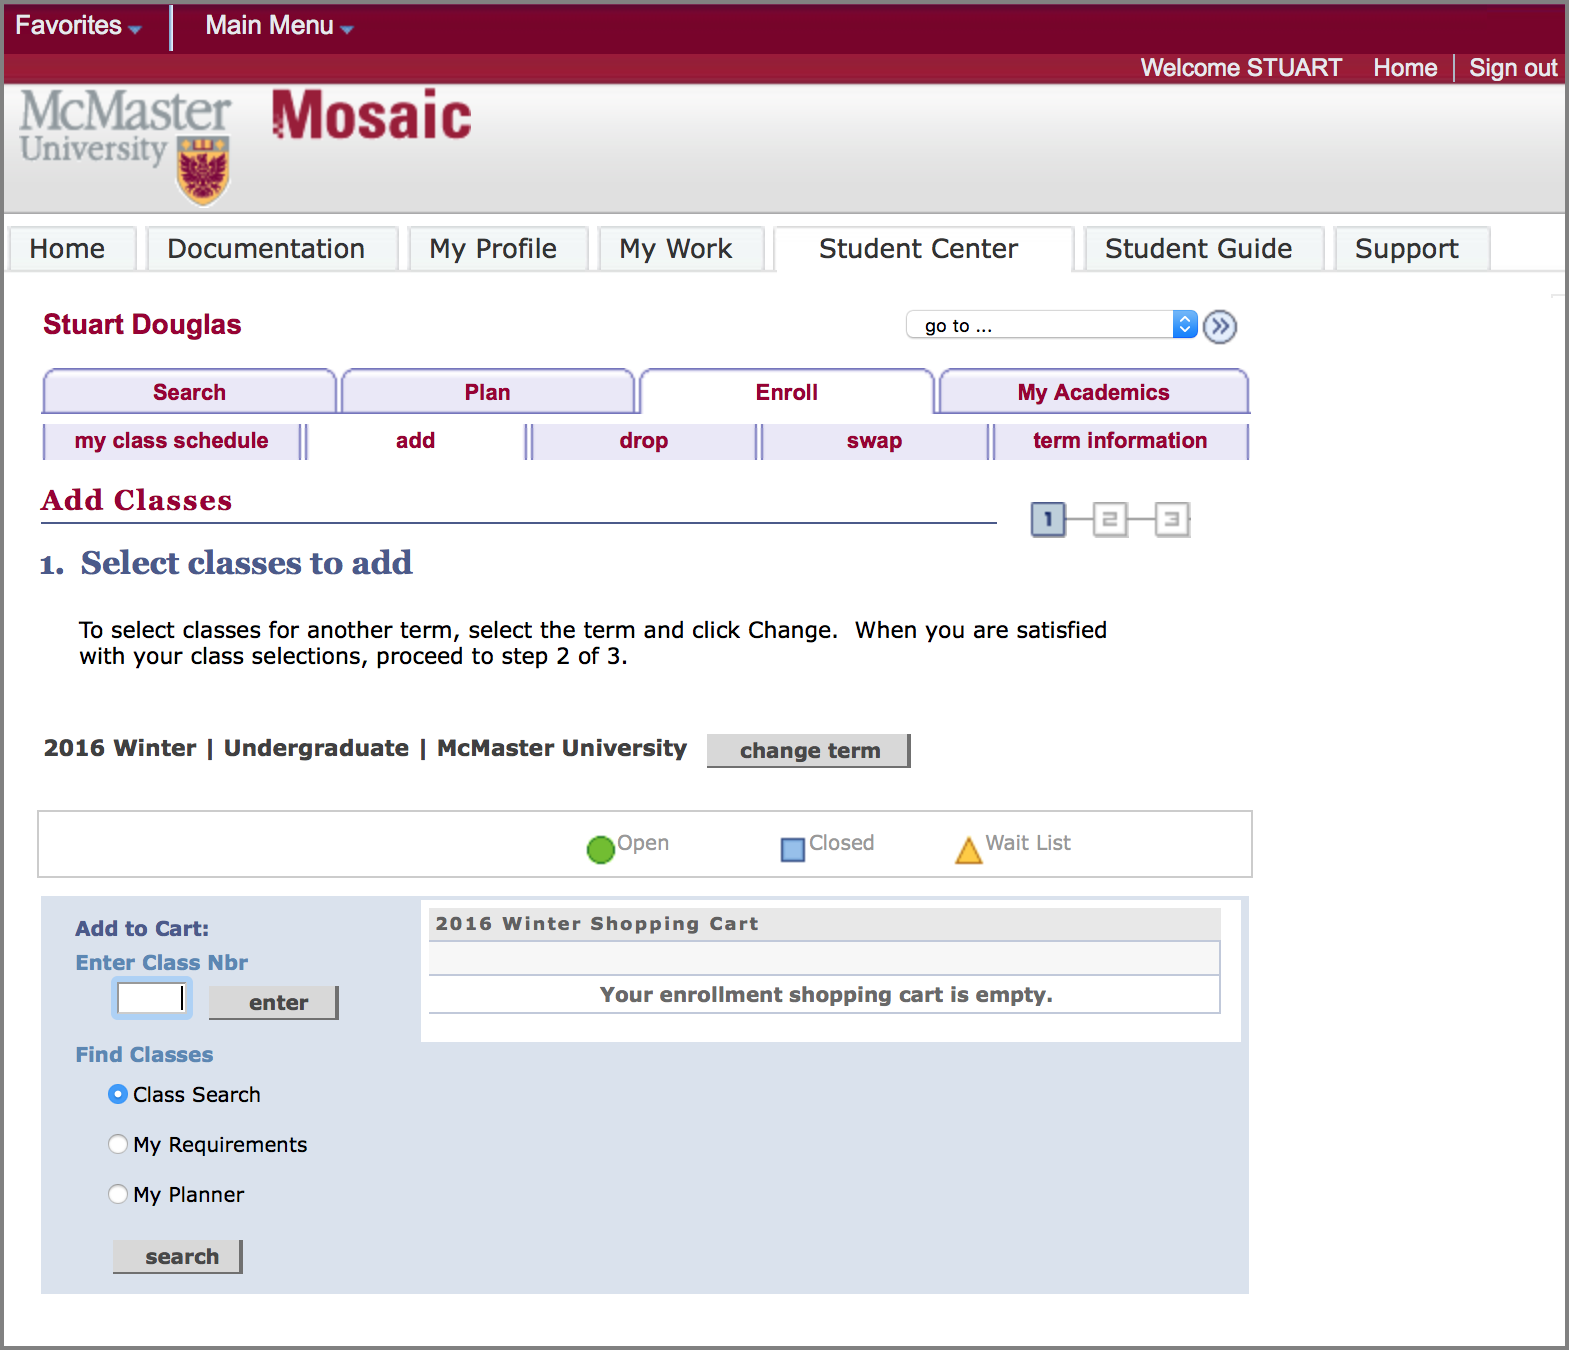
\includegraphics[width=0.9\textwidth]{MosaicScreen.png}
\end{center}
\Caption{Selecting courses to enroll in -- Mosaic}
\end{InlineColumnFigure}

\subsubsection*{Description}
The purpose of the software is to allow students to manage their courses (enrolling, dropping etc.), and view information about their current status (current timetable, enrollment status, financial balance etc.). The interface for the software consists of several distinct modules encapsulating different aspects of the software. These include Academics, Finances, Personal Information, and Admissions. The focus of this analysis is on two common tasks -- enrolling in courses and viewing one's course schedule.

\subsubsection*{Critique}
The largest usability flaws in Mosaic center around difficulty to access required information. Combined with an unintuitive and inconsistent navigation interface, the software is not very usable. The HTA for enrolling in a course demonstrates this through the large number of steps required to perform a routine and common task. Other functions are hidden behind dropdown menus, and are difficult to discover.\\

The navigation is separated into a top navigation bar separated by user-type (e.g. Students and Employees). Within the student center page, functions are separated into modules, an effective strategy to group related functions. Navigating to one of the sub-functions (such as enrolling in a course) presents secondary and tertiary menus below the main one. Navigation within one of these is handled by blue text hyperlinks back to previous pages. Native back and forward browser functionality does not work. There is little visual indication of where the user is beyond the navigation bars at the top, which do not go to a depth sufficient to cover all pages used when performing common actions, such as enrolling in a course.

% =================== SubSection =================== %
\subsection*{McMaster University (pre 2015) -- Solar}
\subsubsection*{Description}
Nam consectetuer. Sed aliquam, nunc eget euismod ullamcorper, lectus nunc ullamcorper orci, fermentum bibendum enim nibh eget ipsum.

\subsubsection*{Critique}
Donec porttitor ligula eu dolor. Maecenas vitae nulla consequat libero cursus venenatis. Nam magna enim, accumsan eu, blandit sed, blandit a, eros.

% =================== SubSection =================== %
\subsection*{Guelph University -- WebAdvisor}
\begin{InlineColumnFigure}
\begin{center}
	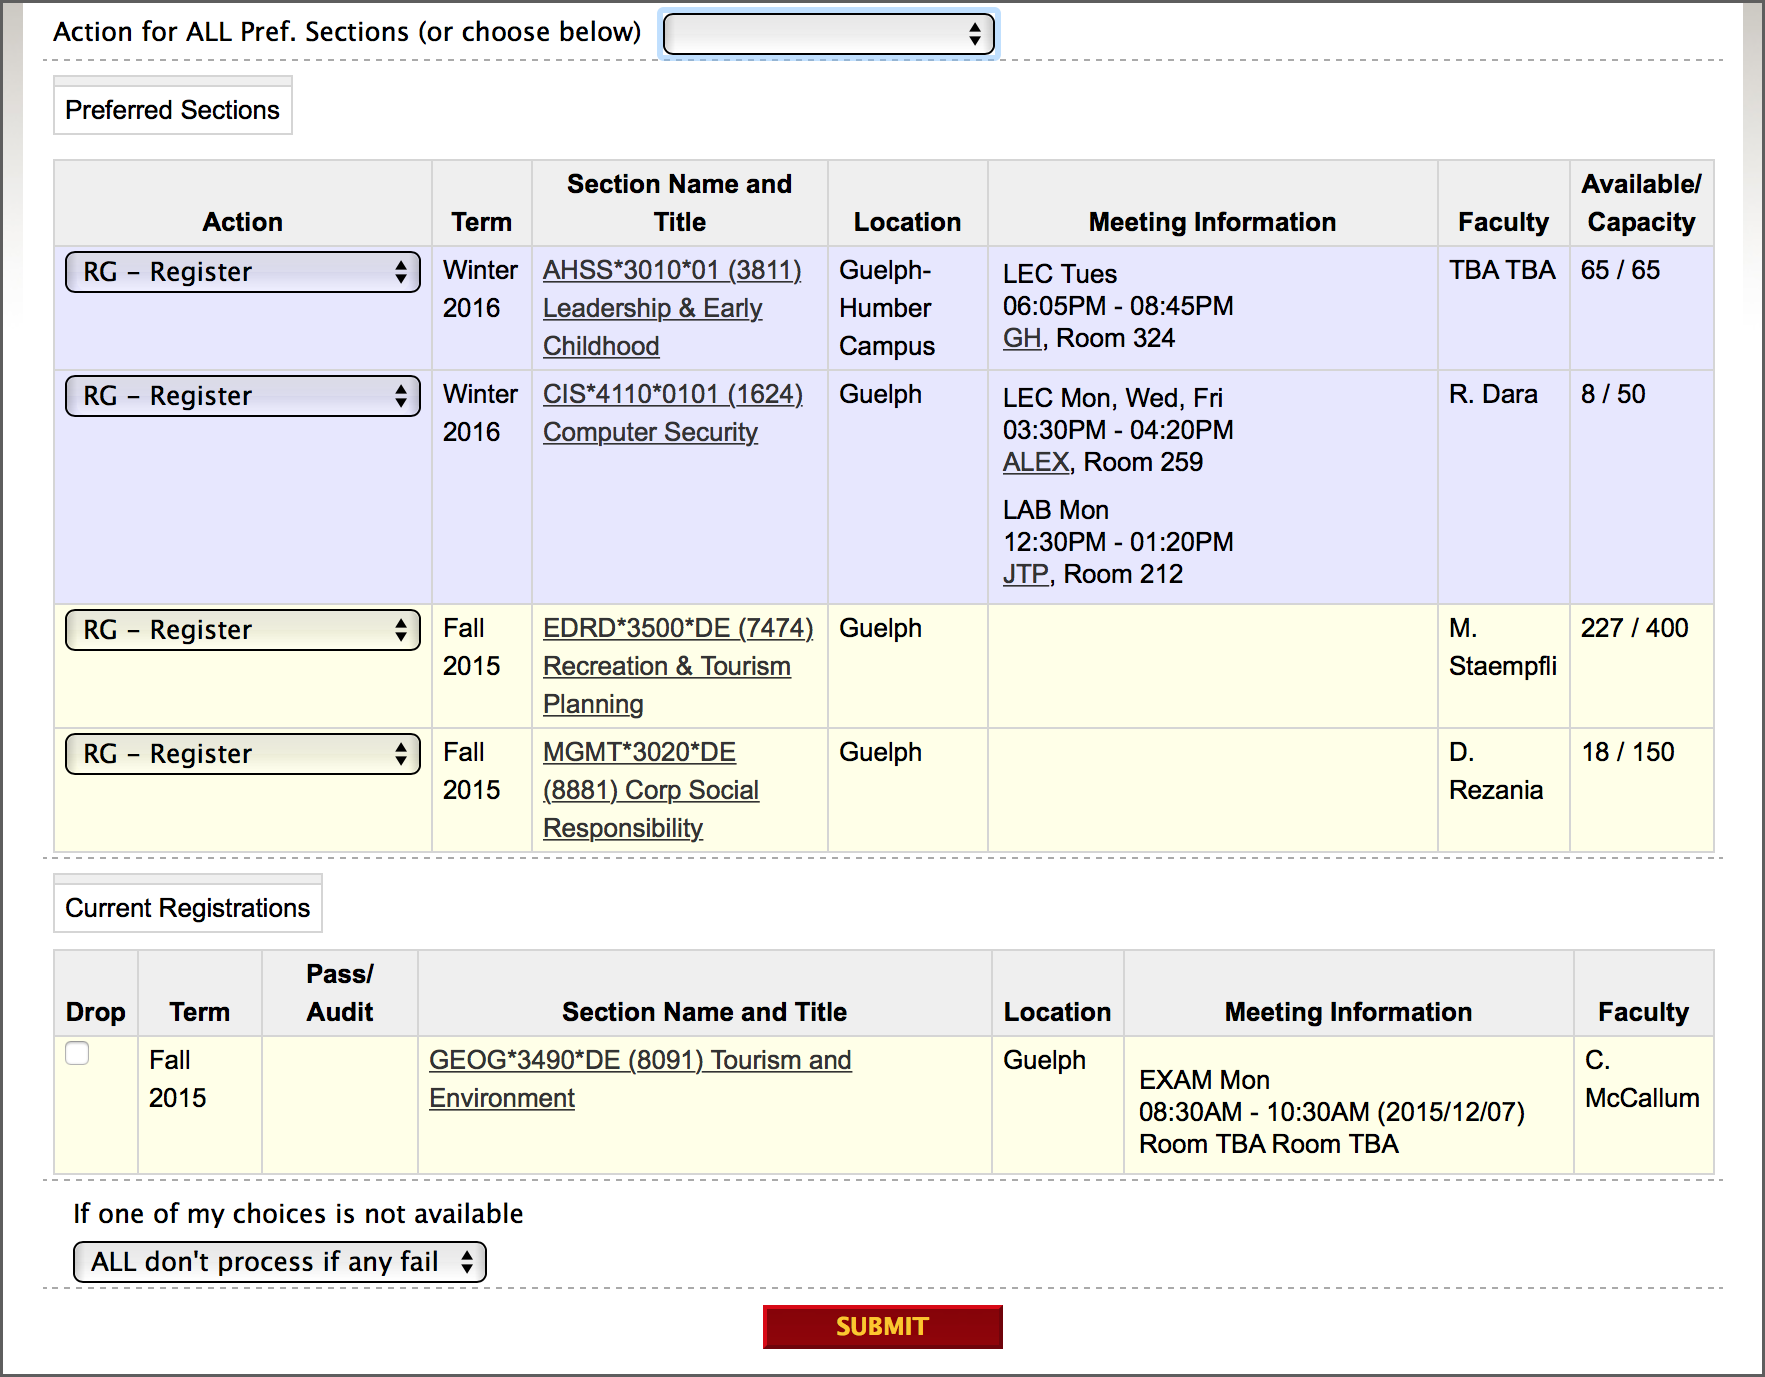
\includegraphics[width=0.9\textwidth]{GuelphScreen.png}
\end{center}
\Caption{Registering for preferred courses -- WebAdvisor}
\end{InlineColumnFigure}

\subsubsection*{Description}
Guelph's

\subsubsection*{Critique}
Aliquam erat volutpat. Sed quis velit. Nulla facilisi. Nulla libero. Vivamus pharetra posuere sapien. 

% =================== SubSection =================== %
\subsection*{Carleton University -- ??}
\subsubsection*{Description}
Nam consectetuer. Sed aliquam, nunc eget euismod ullamcorper, lectus nunc ullamcorper orci, fermentum bibendum enim nibh eget ipsum. 

\subsubsection*{Critique}
Donec porttitor ligula eu dolor. Maecenas vitae nulla consequat libero cursus venenatis. Nam magna enim, accumsan eu, blandit sed, blandit a, eros.

% =================== SubSection =================== %
\subsection*{Waterloo University -- ??}
\subsubsection*{Description}
Lorem ipsum dolor sit amet, consectetuer adipiscing elit. Morbi commodo, ipsum sed pharetra gravida, orci magna rhoncus neque, id pulvinar odio lorem non turpis. 

\subsubsection*{Critique}
Nullam sit amet enim. Suspendisse id velit vitae ligula volutpat condimentum. Aliquam erat volutpat. Sed quis velit. Nulla facilisi. Nulla libero. Vivamus pharetra posuere sapien. 

% =================== Section =================== 
\section*{Conclusion}
We have discussed our proposed improvements to a course management system like mosaic. We also provided a software survey for five Canadian university course management systems. For each survey we critiqued the software as well as analyzed the two most important features via hierarchical task analysis.

\end{multicols}

\newpage
\section*{HTA - Mosaic, Enrolling in a Course}
\begin{center}
\fbox{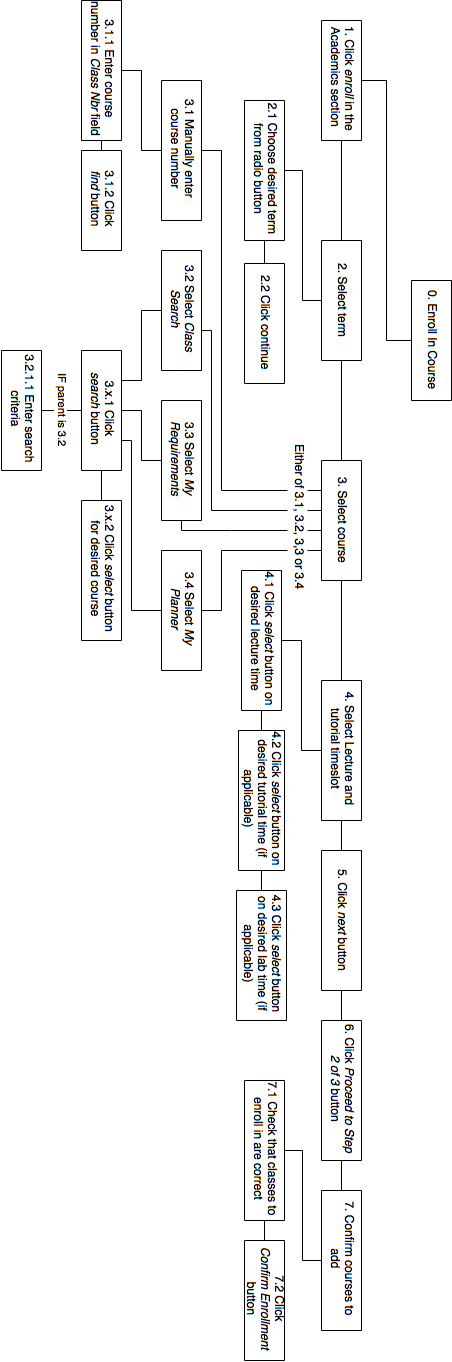
\includegraphics[width=3in]{MosaicEnroll.png}}
\end{center}

\newpage
\section*{HTA - Mosaic, Viewing Weekly Schedule}
\begin{center}
\fbox{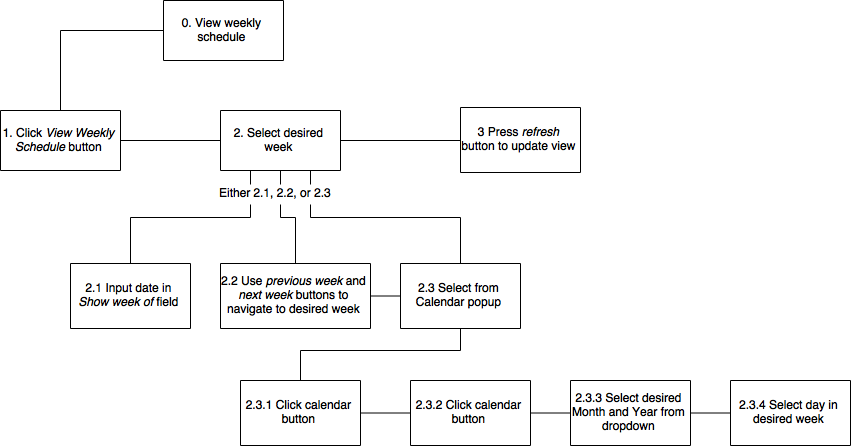
\includegraphics[width=\textwidth]{MosaicViewSchedule.png}}
\end{center}

\vspace{3mm}
\section*{HTA - WebAdvisor, Enrolling in a Course}
\begin{center}
\fbox{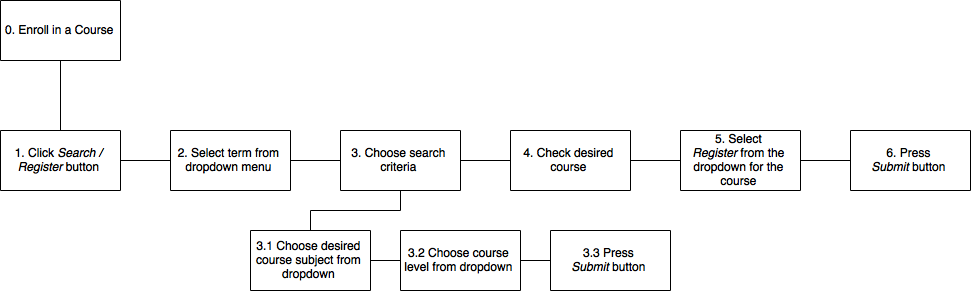
\includegraphics[width=\textwidth]{WebAdvisorEnroll.png}}
\end{center}

\vspace{3mm}
\section*{HTA - WebAdvisor, Viewing Weekly Schedule}
\begin{center}
\fbox{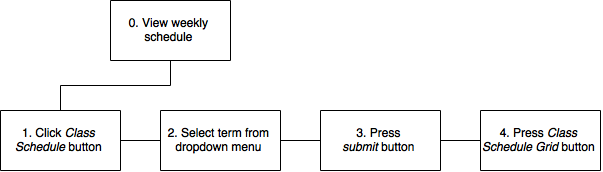
\includegraphics[width=\textwidth]{WebAdvisorViewSchedule.png}}
\end{center}


\end{document}
